\documentclass[a4paper,10pt, twocolumn]{article}

% Wider margins (compared to default)
\usepackage[margin=2.0cm]{geometry}

% For misc. computations
\usepackage{calc}
\usepackage{enumitem}

% English support (typography and hyphenation)
\usepackage[american]{babel}
\usepackage{csquotes}

% For math
\usepackage{amsmath}

% Unicode encoding
\usepackage[utf8]{inputenc}

% Color box
\usepackage{tikz,lipsum,lmodern}
\usepackage[most]{tcolorbox}

% Better default font (Libertine and Inconsolata)
% \usepackage[ttscale=.875]{libertine}
% \usepackage[scaled=0.96]{zi4}

\usepackage{mathspec}
\setmainfont{Minion Pro Cond}
\setmathsfont(Digits,Greek,Latin)[Numbers={Proportional}]{Minion Pro}
\setmathrm{Minion Pro}
\setsansfont{MyriadPro-Cond}

\usepackage{nicefrac}

% Biber
\usepackage[backend=biber,
            style=apa,
%            maxcitenames=3,
%            uniquelist=false,
%            maxbibnames=99,
%            apabackref=false,
            apamaxprtauth=99,
            natbib=true]{biblatex}
\DeclareLanguageMapping{american}{american-apa}



% Graphics
\usepackage{graphicx}

% Figure caption
\usepackage[labelsep=period]{caption}
\renewcommand{\captionfont}{\small\sffamily}
\renewcommand{\captionlabelfont}{\small\sffamily\bfseries}

% Hyperref
\usepackage{xcolor}
\definecolor{blendedblue}{rgb}{0.2, 0.2, 0.6}
\definecolor{blendedred}{rgb}{0.8, 0.2, 0.2}
\usepackage[bookmarks=true,
            breaklinks=true,
            pdfborder={0 0 0},
            citecolor=blendedblue,
            colorlinks=true,
            linkcolor=blendedblue,
            urlcolor=blendedblue,
            citecolor=blendedblue,
            linktocpage=false,
            hyperindex=true,
            linkbordercolor=white]{hyperref}
\usepackage{hyperref}
\hypersetup{colorlinks=true}


% Bibliography file
\bibliography{article.bib}

% Headers
\usepackage{fancyhdr}
\pagestyle{fancy}
% \fancyhf{}
\rhead{\footnotesize \sf page \thepage}
\lhead{\footnotesize \sf Rougier et al. 2017
       \textbullet~The ReScience Initiative}
\rfoot{}
\cfoot{}
\lfoot{}

\makeatletter
\renewcommand{\maketitle}{\bgroup\setlength{\parindent}{0pt}
\begin{flushleft}
  \textbf{\huge\@title\\}
  \vspace{5mm}
  \@author
\end{flushleft}\egroup
}
\makeatother


%% \newtcbox{\orcid}{enhanced,nobeforeafter,tcbox raise base,boxrule=0.4pt,top=0mm,bottom=0mm,
%%   right=0mm,left=4mm,arc=1pt,boxsep=2pt,before upper={\vphantom{dlg}},
%%   colframe=green!50!black,coltext=green!25!black,colback=green!10!white,
%%   overlay={\begin{tcbclipinterior}\fill[green!75!blue!50!white] (frame.south west)
%%     rectangle node[text=white,font=\sffamily\bfseries\tiny,rotate=0] {ID} ([xshift=4mm]frame.north west);\end{tcbclipinterior}}}


\usepackage{tikz}
\usetikzlibrary{positioning,shapes,shadows,arrows}
\newcommand{\orcid}[1]{
    \tikz[baseline=-0.5ex]{ 
        \tikzset{lib/.style={
            rectangle split,
            rectangle split parts=2,
            rectangle split horizontal,
            rectangle split part fill={green!75!blue!50!white,green!10!white},
            rectangle split draw splits=false,
            rounded corners=1pt,
            rectangle split part align={right,right},
            draw=green!50!black,
            minimum height=8pt}
        }
        \node[lib] (var){
        \nodepart[text=green!25!black]{two} \footnotesize \href{http://orcid.org/#1}{#1}};
        \node[text=white,font=\sffamily\bfseries\footnotesize,rotate=0] at ([xshift=6pt]var.west) {ID};
    }
}

\title{Long-Term Reproducibility through Replication:\\
       the ReScience Initiative}
\author{%
  \textbf{Nicolas P. Rougier}$^{1,2,3,*}$,
  \textbf{Konrad Hinsen}$^{4,5}$,
  \textbf{Thomas Arildsen}$^{?}$,
  \textbf{Lorena Barba}$^{?}$,
  \textbf{Fabien Benureau}$^{?}$,
  \textbf{C. Titus Brown}$^{?}$,
  \textbf{Georgios Detorakis}$^{?}$,
  \textbf{Emmanuelle Gouillart}$^{?}$,
  \textbf{Pierre de Buyl}$^{?}$,
  \textbf{Benoît Girard}$^{?}$,
  \textbf{Olivia Guest}$^{?}$,
  \textbf{Mehdi Khamassi}$^{?}$,
  \textbf{Etienne Roesch}$^{?}$,
  \textbf{Joseph Stachelek}$^{?}$,
  \textbf{Owen Petchey}$^{?}$,
  \textbf{Timothée Poisot}$^{?}$,
  \textbf{Karthik Ram}$^{?}$,
  \textbf{Yoav Ram}$^{?}$
  \textbf{Federico Vaggi}$^{?}$,
  \textbf{Julien Vitay}$^{?}$,
  \textbf{Tiziano Zito}$^{?}$\\
  \begin{footnotesize}
    $^{1}$INRIA Bordeaux Sud-Ouest
          Talence, France
    $^{2}$Institut des Maladies Neurodégénératives, Université de Bordeaux,
          CNRS, UMR 5293, Bordeaux, France
    $^{3}$LaBRI, Université de Bordeaux, Institut Polytechnique de Bordeaux,
          CNRS, UMR 5800, Talence, France
    $^{4}$Centre de Biophysique Moléculaire,
          CNRS UPR4301, Orléans Cedex 2
    $^{5}$Synchrotron SOLEIL, Division Expériences,
          Gif sur Yvette, France\\
    $^{*}$Corresponding author:
          \href{mailto:Nicolas.Rougier@inria.fr}{Nicolas.Rougier@inria.fr}          
  \end{footnotesize}
}

\date{}

\begin{document}

\twocolumn[
\maketitle
\begin{small}
  \noindent
  \textbf{} \par
  \textbf{Keywords:} Open Science, Computational Science,
                     Reproducibility, Replicability
\end{small}
\vspace{10mm}
]


\section*{Introduction}
There is a replication crisis in Science. It has been recently highlighted in
medicine \citep{ioannidis:2005}, in psychology \citep{nosek:2015}, in
political sciences \citep{janz:2015} and even more recently in biomedical
sciences \citep{iqbal:2016}. The reasons for such non-reproducibility are as
diverse as these domains can be. In medicine, the {\em study power and bias, the
number of other studies on the same question, and, importantly, the ratio of
true to no relationships among the relationships probed in each scientific
field} are important criterion as reported by \citep{ioannidis:2005}. In psychology,
the infamous p-value seems to be the root of all evil while in biomedical
sciences, \citep{iqbal:2016} identified a {\em lack of access to full datasets and
detailed protocols for both clinical and non-clinical biomedical
investigation}. Surprisingly enough, computational sciences (in the broad
sense) and computer sciences are no exception even though they rely mostly on
code and data that are assumed to be not prone to the aforementioned
problems.\\

When \citep{collberg:2014, collberg:2015} decided to measure precisely the
extent of the problem, they investigated the availability of the code and data,
and {\em the extent to which this code would actually build with reasonable
  effort}. The results were dramatic: on the 515 potentially reproducible
papers (out of 613) targeted by the study, authors managed to ultimately run
only 102 of them. Less than 20\%. It is to be underlined that authors only
studied the possibility to run the code. They did not even check for the
correctness of the code (does the code actually implements what is advertised
in the paper) nor the replicability of the results (does the run lead to the
same results as in the paper).  \citep{topalidou:2015a} encountered the same
problem when they tried to replicate a model from the computational
neuroscience literature: source code were not part of the supplementary section
of the paper and no link nor repository were given in the main text. When they
finally get their hands on the code (after contacting the corresponding
author), it was only to realize it cannot be compiled and was mostly
unusable.\\

Confronted to the problem, a small but growing number of journals and
publishers have decided to react and have adopted explicit data and software
policies. See for example the Plos
\href{http://journals.plos.org/plosone/s/materials-and-software-sharing}{Materials
  and Software Sharing} and
\href{http://journals.plos.org/plosone/s/data-availability}{Data Availability}
or the
\href{https://elifesciences.org/elife-news/inside-elife-forking-software-used-elife-papers-github}{recent
  annoucement} by eLife on forking software used in eLife papers to GitHub.
Such policy will guarantee access to code and data in a proper format
\citep{perkel:2016} but this won't guarantee reproducilbility nor
correctness. At the educational level, things have started to change with a
growing literature on best practices for making code reproducible
\citep{sandve:2013, crook:2013, wilson:2014, halchenko:2015, janz:2015,
  hinsen:2015}. Original initiative such as software and data carpentry
\citep{wilson:2016} are worth to be mentionned since their goal is {\em to make
  scientists more productive, and their work more reliable, by teaching them
  basic computing skills}. Obviously, such best practices could be as well
applied to already published research software or code, provided the original
author(s) is willing to take the challenge of re-implementing his/her own
software for the sake of Science. This is unlikely since, unfortunately, the
incentives for doing such a time-consuming task are low or nonexistent.
Furthermore, if the original author did some mistake in his/her original
implementation, chances are that he/she'll reproduce the same mistake over and
over again (just an educated guess, we have no data supporting this
assertion).\\

%% At this point, the question is what do we do? Do we have to declare
%% the research to be lost once and for all because the associated software or
%% code is nowhere to be found / lost / damaged / malfunctioning / not runnable /
%% not usable / does not give original results / etc. We would doom ourselves by
%% doing so

% As you may have guessed by now, this was the main motivation for
 %the creation of the ReScience journal\citep{^2].

\section*{Reproducibility is harder than you think}

\citeauthor{Mesnard:2016} explains in \citep{Mesnard:2016} that writing
reproducible and replicable computational fluid dynamics simulation is harder
than you think. In fact, there are several different reasons for
non-reproducibility that, for the most part, largely depends on the specific
scientifc domain. However, from our publishing experience, there are also some
common behaviors that can be identified. Missing code and/or data, unknown
dependencies, inaccurate or imprecise description appears to be shared
characteristics of a lot of work.\\

To be extended...

\section*{The ReScience initiative}

Writing a replication might be a daunting task that is usually hardly or not
rewarded. Nevertheless, some people are actually willing to replicate
computational research. The motivation for doing so is very diverse and range
from the simple student who want to train oneself in order to get familiar with
a specific scientific domain up to the senior researcher that has a critical
need of a specific piece of code (see Box 1). If these people write a brand new
open source implementation of some published research, chances are this new
implementation may be of great interest for other people as well, includign
original authors. The question is where to publish such replication. To the
best of our knowledge, no journal would accept to publish a single successful
replication in computational science. This has been the main motivation for the
creation of the ReScience journal (\url{rescience.github.io}) by Konrad Hinsen
and Nicolas Rougier in 2015.\\

\begin{tcolorbox}[breakable, pad at break*=1mm,
                  colback=black!2.5, arc=0pt, outer arc=0pt, boxrule=0pt]
\begin{footnotesize}
\textbf{Box 1.} Authors having  published in Rescience explain their motivation.\\

\textbf{(\cite{stachelek:2016})} I was motivated to replicate the results of
the original paper because I feel that working through code supplements to blog
posts has really helped me learn how to science. I could have published my
replication as a blog post but I wanted the exposure and permanency that goes
along with journal articles. This was my first experience with formal
replication. I think the review was useful because it forced me to consider how
the replication would be used by people other than myself. I have not yet
experienced any new interactions following publication. However, I did notify
the author of the original implementation about the replication's
publication. I think this may lead to future correspondence. The original
author suggested that he would consider submitting his own replications to
ReScience in the future.\\

\textbf{(\cite{topalidou:2015b})} Our initial motivation and the main reason
for replicating the model is that we needed it in order to collaborate with our
neurobiologist colleagues. When we arrived in our new lab, the model has just
been published (2013) but the original author left the lab a few months before
our arrival. There were no public repository, no version control and the paper
describing the model was incomplete and partly inaccurate. We managed to get
our hands on the original sources (6,000 lines of Delphi) only to realize we
could not compile them. It took us three months to replicate it using 250 lines
of Python. But at this time, there were no place to publish this kind of
replication and share the new code with colleagues. Since then, we have refined
the model and made new predictions that have been confirmed. Our initial
replication effort really gave the model a second life.\\

\textbf{(\cite{viejo:2016})} Replicating previous work is a relatively routine
task every time we want to build a new model: either because we want to build
on it, or because we want to compare to it. We also give replication tasks to
M.Sc. students every year, as projects. In all these cases, we are confronted
to incomplete or inaccurate model descriptions, as well as to the impossibility
to obtain the original results. Contacting the original authors sometimes
solves the problem, but not so often (because of the {\em dog ate my hard
  drive} syndrom). We thus accumulate knowledge, internal to the lab, about
which model work, which doesn't, and how a given model has to be parameterized
to really work. Without any place to publish it, this knowledge is
wasted. Publishing it in ReScience, opening the discussion publicly, will be a
progress for all of us. \par
\end{footnotesize}
\end{tcolorbox}

ReScience is an open peer-reviewed journal that targets computational research
and encourages the explicit replication of already published research,
promoting new and open-source implementations in order to ensure that the
original research is reproducible. In less than two years of existence, 12
articles have been published and 3 are currently under review
(\href{https://github.com/ReScience/ReScience-submission/pull/20}{\#20},
\href{https://github.com/ReScience/ReScience-submission/pull/27}{\#27},
\href{https://github.com/ReScience/ReScience-submission/pull/30}{\#30}). The
editorial board covers a wide range of computational sciences (see
\url{http://rescience.github.io/board/}) and there are more than 70 registered
reviewers that have volunteered. The computational domains of published work
are in computational neuroscience, neuroimaging, computational ecology and
computer graphics with a majority in computational neuroscience. There is a
strong bias in favor of successful replication (100\%) and experience has
taught us researcher are reluctant to publish a failed replication (even when
there is a way to prove the original work is wrong). For a young researcher,
there is a social/professional risk in publishing an article where he/she shows
that the results from a senior researcher are wrong. Until we implement a
certified anonymized submission process, this strong bias will most likely
remain.\\

One of the specificity of the ReScience journal is its publishing chain that is
radically different from any other traditional scientific journals since
ReScience lives on GitHub. Each submission takes the form of a pull request
that is first considered by a member of the editorial board, who may decide to
reject the submission, or assign it to two reviewers for further review and
tests. The reviewers evaluate the code and the accompanying material in
continuous interaction with the authors through the discussion section. If both
reviewers managed to run the code and obtain the same results as the ones
advertised in the accompanying material, the submission is
accepted. Furthermore, an author cannot submit a replication of his/her own
research, nor the research of close collaborators. Mistakes in the
implementation of research questions and methods are often due to biases
authors invariably have, consciously or not. One's biases will inevitably carry
over to how one approaches a replication. Perhaps even more importantly, this
aims at the cross-fertilization of research and trying to replicate the work of
one’s peers might pave the way for a future collaboration, or may give rise to
new ideas as a result of the replication effort.\\

The main criterion for acceptation is the actual replication of the research
with a clear statement by the authors explaining why they think they have
replicated the paper (same figures, same graphics, same behavior,
etc.). However, the clarity of the code is an important criterion because
uncommented or obfuscated code is as bad as no code at all. A code without the
accompanying article is also a criterion for rejection since we’re not human
compilers (well not all of us at least). The role of the reviewer is thus to
ensure the proposed submission is actually replicable. This means:
%
\begin{itemize}
\item One should be able to run the proposed implementation on hi/her computer
\item One should obtain the same results as indicated in the accompanying paper
\item These results must correspond to the original paper
\end{itemize}
%
The goal of the review is thus to help the author to meet ReScience quality
standards through discussion. More specifically, since ReScience targets
replication of original research, there is no need to judge the relevance or
novelty of the research. The review concentrates on how easy it would be for
another researcher to run the proposed implementation. This should be viewed in
light of the standards in the field. If a given tool/library/software is
mainstream in a field, it is ok to use them, but if a brand new standalone
implementation is proposed, this must not rejected on this criterion.


%% It has been said many times by many authors in the litterature that
%% reproducibility is the cornerstone of Science and we, as a scientific
%% community, should aim at such reproducibility. However, good intention are not
%% sufficient and a given computational results can be declared reproducible if
%% and only if it has been actually replicated in a the sense of a brand new
%% open-source and documented implementation.

%% ReScience already published 4 articles and as shown above, the original
%% motivations of these authors are all different and this might become even more
%% obvious and diverse with future publications. But, beyond these motivations,
%% publishing in ReScience may be especially important for students since this
%% represent a unique opportunity to show the community a given student is able to
%% read a scientific article, to have a deep understanding of it, to write a new
%% implementation and to eventually write a scientific article describing his/her
%% work. Although the ReScience publishing model is a bit different from other
%% academic journals, it can give students a first experience at peer-reviewed
%% scholarly publishing, including meeting standards of scientific rigor and
%% addressing reviewers' comments.  Furthermore, publishing in ReScience is a way
%% to actively contribute to open science while adding to one's publication
%% record.

%\Discussion*{Discussion}
%\subsection*{An Utopia for Tomorrow}

\begin{figure}
  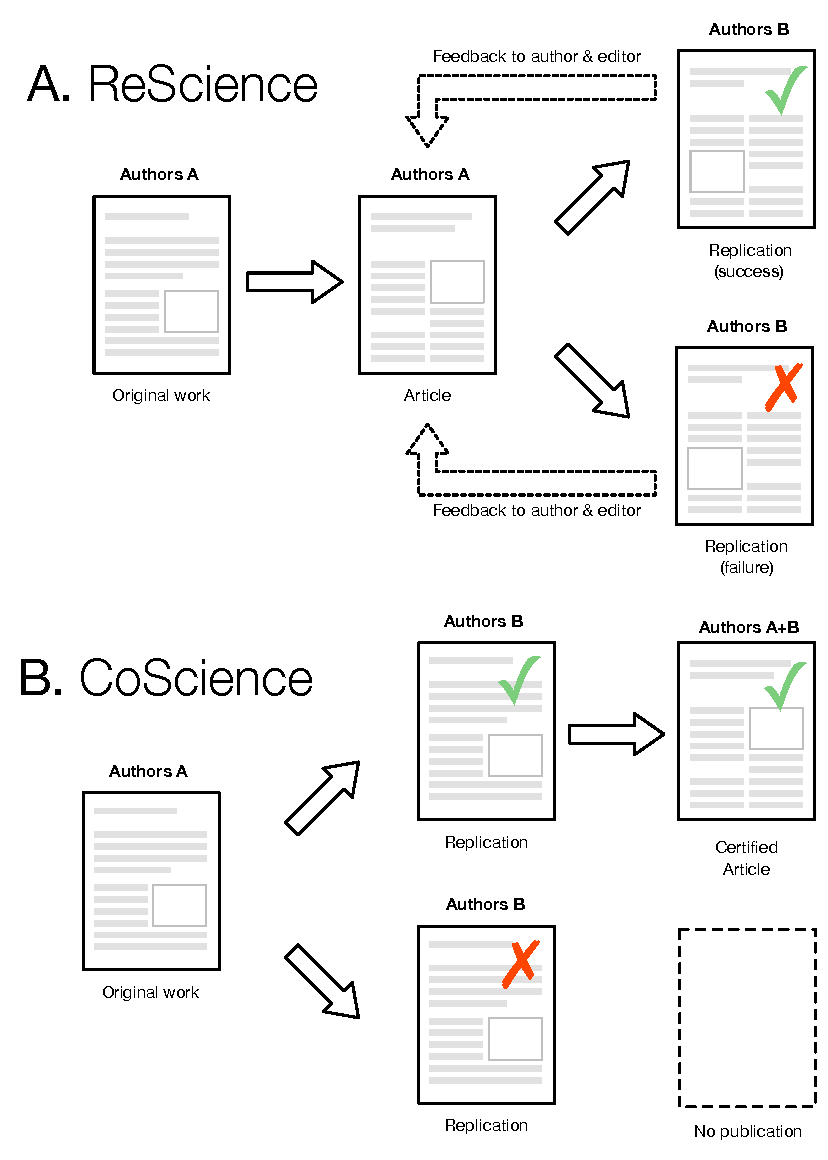
\includegraphics[width=1.0\columnwidth]{CoScience}
  \caption{\textbf{A} The ReScience publication chain starts from an original
    research by authors A, published in a journal, in proceedings or as a
    preprint. This article constitutes the base material for authors B that
    will attempt to replicate the work based on its description. Success or
    failure to replicate is not a criterion for rejection even though failure
    to replicate will requires more precaution to ensure this is not a
    misunderstanding or a bug in the new code. After review and once published,
    a feedback is given to original author and editor to inform them the work
    has been replicated (or not). \textbf{B} The CoScience proposal would
    require for the replication to happen before the actual publication. In
    case of failure, nothing will be published, in case of success, the
    publication will be endorsed by authors A and authors B with identified
    roles and will be certified as reproducible because it has beenactually
    replicated by an independent group.}
\end{figure}


\section*{Discussion}

% -> Short-term vs long-term reproducibility
The code accompanying a ReScience replication ensures only a short term
reproducibility. Even if a piece of code is written enforcing best practices,
is reviewed and tested, it suffers from the same problem as any other piece of
code, i.e. it depends on a software stack whose stability is not guaranteed in
the long term. \citep{Mesnard:2016} illustrated this problem very clearly when
they tried to reproduce their own work two years apart. Even though Barba's
group is committed to reproducible software, they did not escape the many
problems one can face when trying to re-run a piece of code. This means the
newly produced code for ReScience will be deprecated at some point in the
future. It can be a matter of months or years (or even decades), but in the
end, it will be deprecated. However, the long-term value of a ReScience
publication is not the actual code but the accompanying article. If you
consider the original article with missing or incomplete information and the
new article with missing and checked information, you have a complete and
consistent description of the original work. This means than 5, 10 or 20 years
from now, one should be able to replicate the work thanks to these two
articles. Of course, the new code can also help, but the true value of a
replication is the accompanying article.

% -> Long term storage: Software Heritage

% -> Computational vs Experimental: ReScience X (Etienne Roesch)

% -> Post vs Pre replication: CoScience, an utopia for tomorrow


% -------------------------------------------------------------- References ---
\renewcommand*{\bibfont}{\footnotesize}
\printbibliography[title=References]


\end{document}

